% Created 2013-02-20 Wed 15:29
\documentclass{article}
\usepackage[utf8]{inputenc}
\usepackage{fixltx2e}
\usepackage{url}
\usepackage{graphicx}
\usepackage{minted}
\usepackage{color}
\usepackage{longtable}
\usepackage{float}
\usepackage{wrapfig}
\usepackage{soul}
\usepackage{textcomp}
\usepackage{amsmath}
\usepackage{marvosym}
\usepackage{wasysym}
\usepackage{latexsym}
\usepackage{amssymb}
\usepackage[linktocpage,
  pdfstartview=FitH,
  colorlinks,
  linkcolor=blue,
  anchorcolor=blue,
  citecolor=blue,
  filecolor=blue,
  menucolor=blue,
  urlcolor=blue]{hyperref}
\usepackage{attachfile}
\tolerance=1000
\providecommand{\alert}[1]{\textbf{#1}}

\title{Homework 2 - Due 2/20/2013}
\author{John Kitchin}
\date{2013-02-13 Mon}
\hypersetup{
  pdfkeywords={},
  pdfsubject={},
  pdfcreator={Emacs Org-mode version 7.9.3a}}

\begin{document}

\maketitle


\section{Calculate the number of atoms/cm$^{2}$ in the following surfaces:}
\label{sec-1}


a) FCC(100) Cu, Pt

b) FCC(111) Cu, Pt

c) BCC(100) Mo,W

d) BCC(110) Mo, W
\subsection{Solution \textbf{:solution:}}
\label{sec-1-1}
\subsubsection{a)}
\label{sec-1-1-1}

Cu: 3.61 \AA{}
Pt: 3.92 \AA{}

There are 2 atoms on the fcc(100) face, and the area of the face is $a^2$. 1 \AA{} = 1e-10 m


\begin{minted}[frame=lines,fontsize=\scriptsize,linenos]{python}
m = 1
cm = 0.01 * m
Ang = 1e-10 * m 

print 'Cu(100): {0:1.2E} atoms/cm^2'.format(2.0 / (3.61 * Ang / cm)**2)
print 'Pt(100): {0:1.2E} atoms/cm^2'.format(2.0 / (3.92 * Ang / cm)**2)
\end{minted}

\begin{verbatim}
 Cu: 1.53E+15 atoms/cm^2
 Pt: 1.30E+15 atoms/cm^2
\end{verbatim}
\subsubsection{b)}
\label{sec-1-1-2}

We need the area of an fcc(111) unit cell. We can compute this from the primitive lattice vectors, which form a primitive fcc(111) cell containing one atom.


\begin{minted}[frame=lines,fontsize=\scriptsize,linenos]{python}
import numpy as np
m = 1
cm = 0.01 * m
Ang = 1e-10 * m 

a = 3.61
b = a / 2.0

v1 = np.array([0.0, b, b])
v2 = np.array([b, 0.0, b])
A = np.linalg.norm(np.cross(v1, v2))* Ang**2 /(cm**2)

print 'Cu(111): {0:1.2E} atoms/cm^2'.format(1.0 / A)

a = 3.92
b = a / 2.0

v1 = np.array([0.0, b, b])
v2 = np.array([b, 0.0, b])
A = np.linalg.norm(np.cross(v1, v2))* Ang**2 /(cm**2)
print 'Pt(111): {0:1.2E} atoms/cm^2'.format(1.0 / A)
\end{minted}

\begin{verbatim}
 Cu(111): 1.77E+15 atoms/cm^2
 Pt(111): 1.50E+15 atoms/cm^2
\end{verbatim}

The 111 surface is more densely packed than the (100) surface.
\subsubsection{c)}
\label{sec-1-1-3}


Mo = 3.15
W = 3.16

The bcc(100) surface only has one atom in it, and the area is $a^2$.


\begin{minted}[frame=lines,fontsize=\scriptsize,linenos]{python}
m = 1
cm = 0.01 * m
Ang = 1e-10 * m 
print 'Mo(100): {0:2e} atoms/cm^2'.format(1.0 / (3.15**2 *Ang**2 / cm**2))
print 'W(100): {0:2e} atoms/cm^2'.format(1.0 / (3.16**2 *Ang**2 / cm**2))
\end{minted}

\begin{verbatim}
 Mo(100): 1.007811e+15 atoms/cm^2
 W(100): 1.001442e+15 atoms/cm^2
\end{verbatim}
\subsubsection{d)}
\label{sec-1-1-4}


The bcc(110) surface has two atoms in it. The area of the unit cell is $a * \sqrt(2) * a$.


\begin{minted}[frame=lines,fontsize=\scriptsize,linenos]{python}
import numpy as np

m = 1
cm = 0.01 * m
Ang = 1e-10 * m 
print 'Mo(110): {0:2e} atoms/cm^2'.format(2.0 / (3.15**2 * np.sqrt(2) * Ang**2 / cm**2))
print 'W(110): {0:2e} atoms/cm^2'.format(2.0 / (3.16**2 * np.sqrt(2) * Ang**2 / cm**2))
\end{minted}

\begin{verbatim}
 Mo(110): 1.425259e+15 atoms/cm^2
 W(110): 1.416253e+15 atoms/cm^2
\end{verbatim}
\section{In the following image the large blue circles are the surface metal atoms and the small black circles represent adsorbates.}
\label{sec-2}


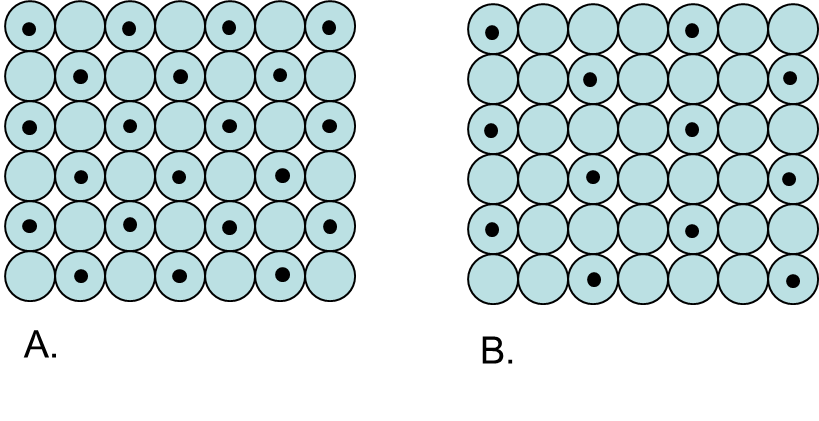
\includegraphics[width=.9\linewidth]{./images/hwk2-leed.png}

a) Give an example of what surface the large circles could represent.

b) Describe the overlayer in each case using matrix notation. If possible, also express the overlayer using Wood's notation.

c) Calculate the reciprocal lattice vectors for each case.

d) Sketch the LEED pattern you expect for these two surfaces.
\subsection{solution \textbf{:solution:}}
\label{sec-2-1}
\subsubsection{a. This could be an fcc or bcc (100) surface.}
\label{sec-2-1-1}
\subsubsection{b)}
\label{sec-2-1-2}

on A: 

\begin{verbatim}
[[1 1]
 [1 -1]]
\end{verbatim}

In Wood's notation, p($\sqrt{2} \times \sqrt{2}) R 45^\circ$

on B:

\begin{verbatim}
[[2 1]
 [0 2]]
\end{verbatim}

This can be described as c(4 \texttimes{} 2)
\subsubsection{c)}
\label{sec-2-1-3}


\begin{minted}[frame=lines,fontsize=\scriptsize,linenos]{python}
import numpy as np

uc1 = np.array([[1, 1], [1, -1]])

print np.linalg.inv(uc1.T)
\end{minted}

\begin{verbatim}
 [[ 0.5  0.5]
  [ 0.5 -0.5]]
\end{verbatim}


\begin{minted}[frame=lines,fontsize=\scriptsize,linenos]{python}
import numpy as np

uc1 = np.array([[2, 1], [0, 2]])

print np.linalg.inv(uc1.T)
\end{minted}

\begin{verbatim}
 [[ 0.5   0.  ]
  [-0.25  0.5 ]]
\end{verbatim}
\subsubsection{d)}
\label{sec-2-1-4}


A)
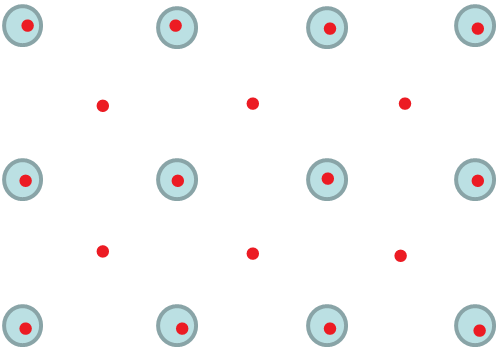
\includegraphics[width=.9\linewidth]{./images/leed-image-1.png}

B)

\includegraphics[width=.9\linewidth]{./images/leed-image-2.png}

\end{document}
